\section{Example: the QR Factorization}
\label{sec:ftla}

In this section, we propose to illustrate the applicability of \cof by
considering a representative routine of a widely used
class of algorithms: dense linear factorizations. The QR factorization
is a cornerstone building block in many applications, including solving
$Ax=b$ when matrices are ill-conditioned, computing eigenvalues, least
square problems, or solving sparse systems through the GMRES iterative
method. For an $M\times N$ matrix $A$, the QR factorization produces $Q$ and
$R$, such that $A=QR$ and $Q$ is an $M\times M$ orthogonal matrix and
$R$ is an $M\times N$ upper triangular matrix. The most commonly used
implementation of the QR algorithm on a distributed memory machine comes
from the ScaLAPACK linear algebra library~\cite{dongarra1997scalapack},
based on the block QR algorithm. It uses a 2D block-cyclic distribution
for load balance, and is rich in level 3 BLAS operations, thereby
achieving high performance.

%$Q$ is stored
%under the lower diagonal of the input matrix in the form of a $WY$
%representation of the Householder transformation
%products~\cite{schreiber1989storage,bischof1985wy}.

\subsection{\abft QR Factorization}

In the context of FT-MPI, the ScaLAPACK QR algorithm has been rendered fault
tolerant through an \abft method in previous work~\cite{pengduppopp12}. This
\abft algorithm protects both the left ($Q$) and right ($R$) factors from fail-stop
failures at any time during the execution.  At the time of failure, every surviving process is notified by FT-MPI. FT-MPI
then spawns a replacement process that takes the same grid coordinates in the
$P\times Q$ block-cyclic distribution. Missing checksums are recovered from
duplicates, a reduction collective communication recovers missing data blocks in
the right factor from checksums. The left factor is protected by the Q-parallel
panel checksum, it is either directly recovered from checksum, or by
recomputing the panels in the current Q-wide section
(see~\cite{pengduppopp12}). Although this algorithm is fault tolerant, it
requires continued service from the MPI library after failures -- which is a
stringent requirement that can be waived with \cof.

\subsection{Checkpoint-on-Failure QR}

\paragraph*{Checkpoint Procedure:} In our current implementation of
\cof, system-level checkpointing is not supported and would result in
restoring the state of the broken MPI library upon restart. Instead, the
application provides a custom MPI error handler, which invokes an
algorithm specific checkpoint procedure to dump the matrices and the
value of important loop indices into a file.

\paragraph*{State Restoration:} In the theoretical version of the \abft
algorithm, regardless of when the failure is detected, the current
iteration is completed before entering the recovery procedure, so that
all updates are applied to the checksums. In the case of the \cof
protocol, failures interrupt the algorithm immediately, the current
iteration cannot be completed due to lack of communication capabilities.
A ScaLAPACK program has a deep call stack, layering functions from
multiple software packages, such as PBLAS, BLACS, LAPACK and BLAS.
Because failure notification happens only in MPI, lower level, local
procedures (BLAS, LAPACK) are never interrupted. However, PBLAS
operations may be incomplete, and therefore checksums only partially
updated.

To resolve this issue, the call stack must be restored on every process.
The current indices in the loop nest of the QR algorithm, down to the
PBLAS level, are adjunct to the checkpoint. When restarted from a
checkpoint, a process undergoes a ``dry run'' phase that mimics the
already completed loop nests, without actually applying modifications to
or exchanging data. When the same loop indices as before the failure are
reached, the matrix content is loaded from the checkpoint; the state is
then identical to that immediately preceding the failure. The regular
\abft recovery procedure can then be applied: the current iteration of
the factorization is completed to update all checksums and the dataset
is finally rebuilt using the \abft reduction.

\begin{comment}
	
A special situation where failure occurs during 
lower level routines such as PDLARFB is also addressed. This critical 
situation has not been  
covered by any previous work for the complexity it introduces.
	
\subsection{Failure in PBLAS routines}
An important condition for the effectiveness of \abft is the
completion of the current iteration. When a failure interrupts the
program execution during an iteration, the checksum ends up in
intermediate form and as a result cannot be used for recovery.  This
problem worsens when a failure occurs during a lower level routine, 
like a PBLAS, causing a partial trailing matrix update. In this case, updates have been applied to parts of the dataset, possibly without having updated accordingly the corresponding checksums. In the case of the QR algorithm, this problem
is solved by saving the local state when a failure is detected in
PDLARFB rather than in PDGEQRF. The recovery
process in this case is described as follow.

\begin{figure}[b]
	\centering
	\subfigure[After the first step: $A_{2}^{T}V$]{\label{fig:gull1}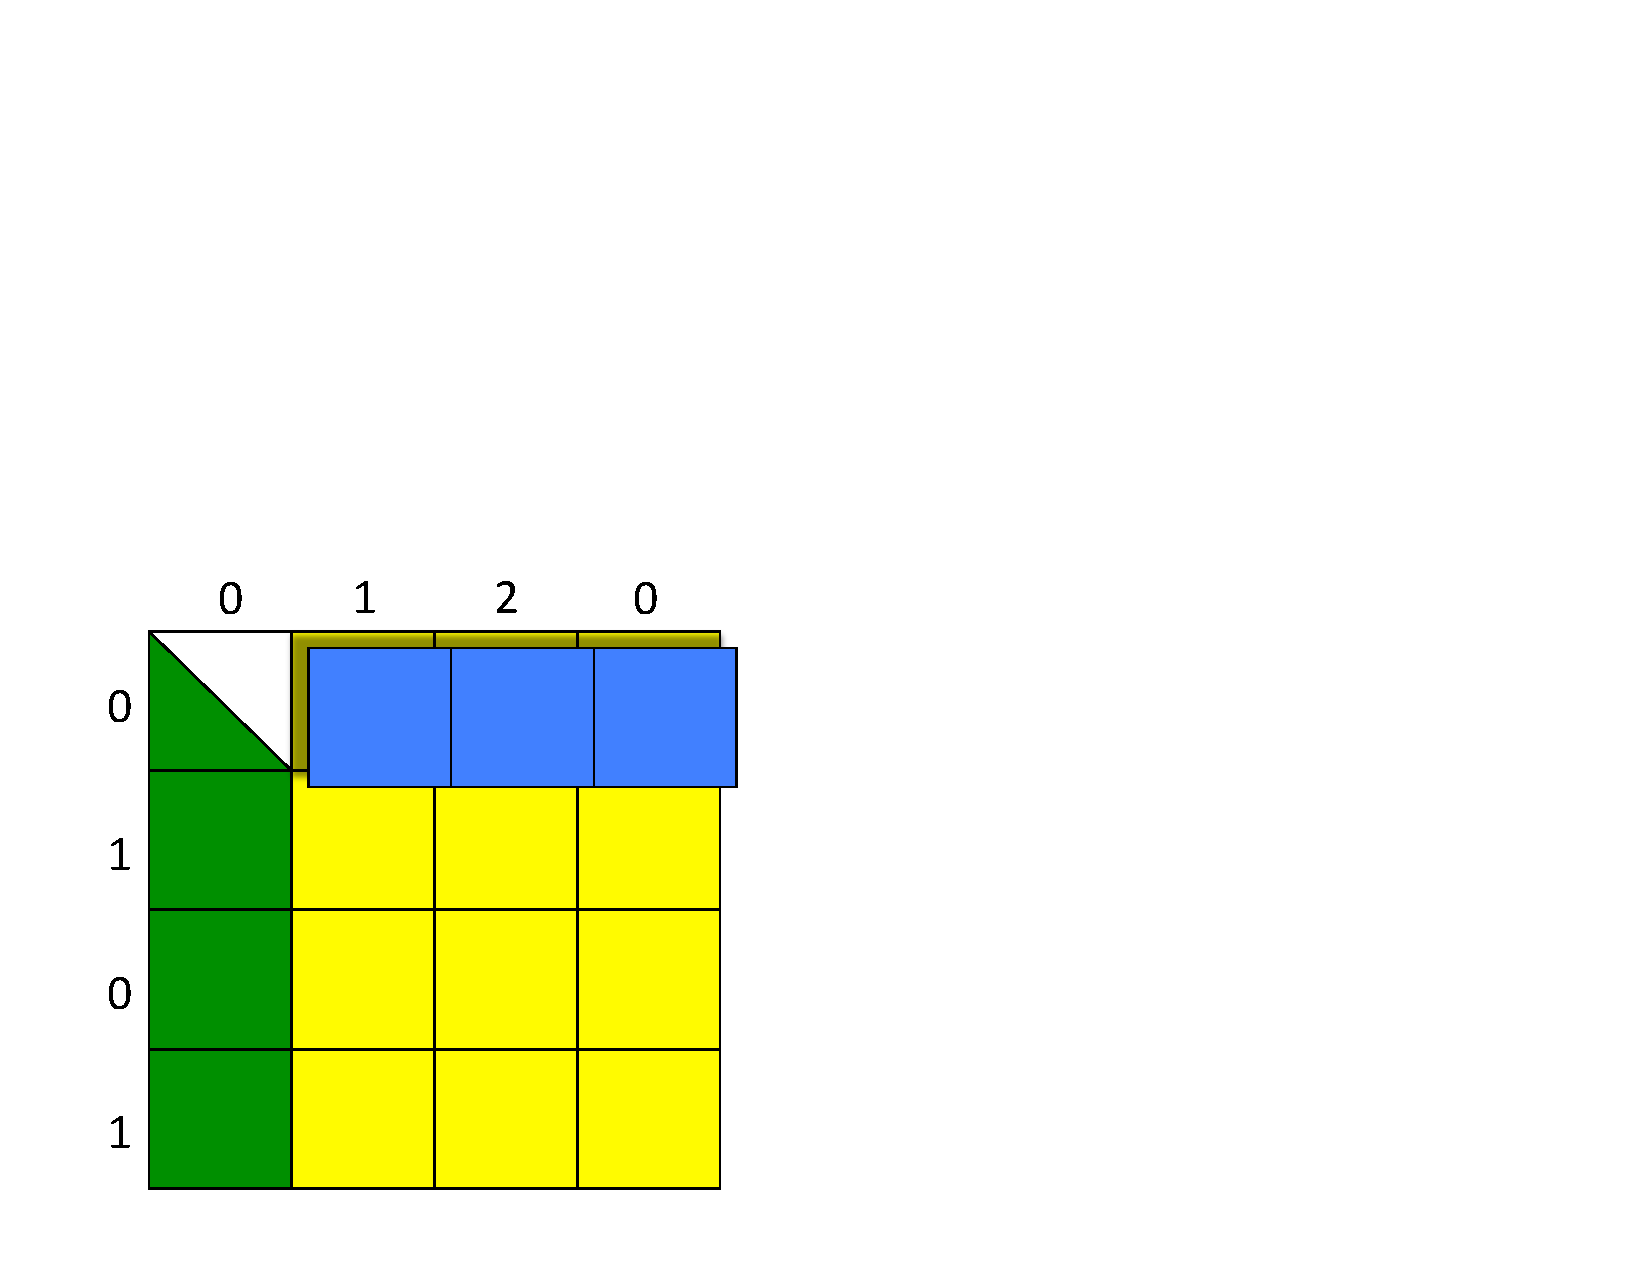
\includegraphics[totalheight=0.15\textheight, width=0.18\textwidth,viewport=10 10 360 360, clip]{figures/pdlarfb_step1}
	\label{fig:pdlarfb_step1}}
	%\line(0,1){100}
	\subfigure[$A_{2}-V\tilde{W}^{T}$]{\label{fig:gull2}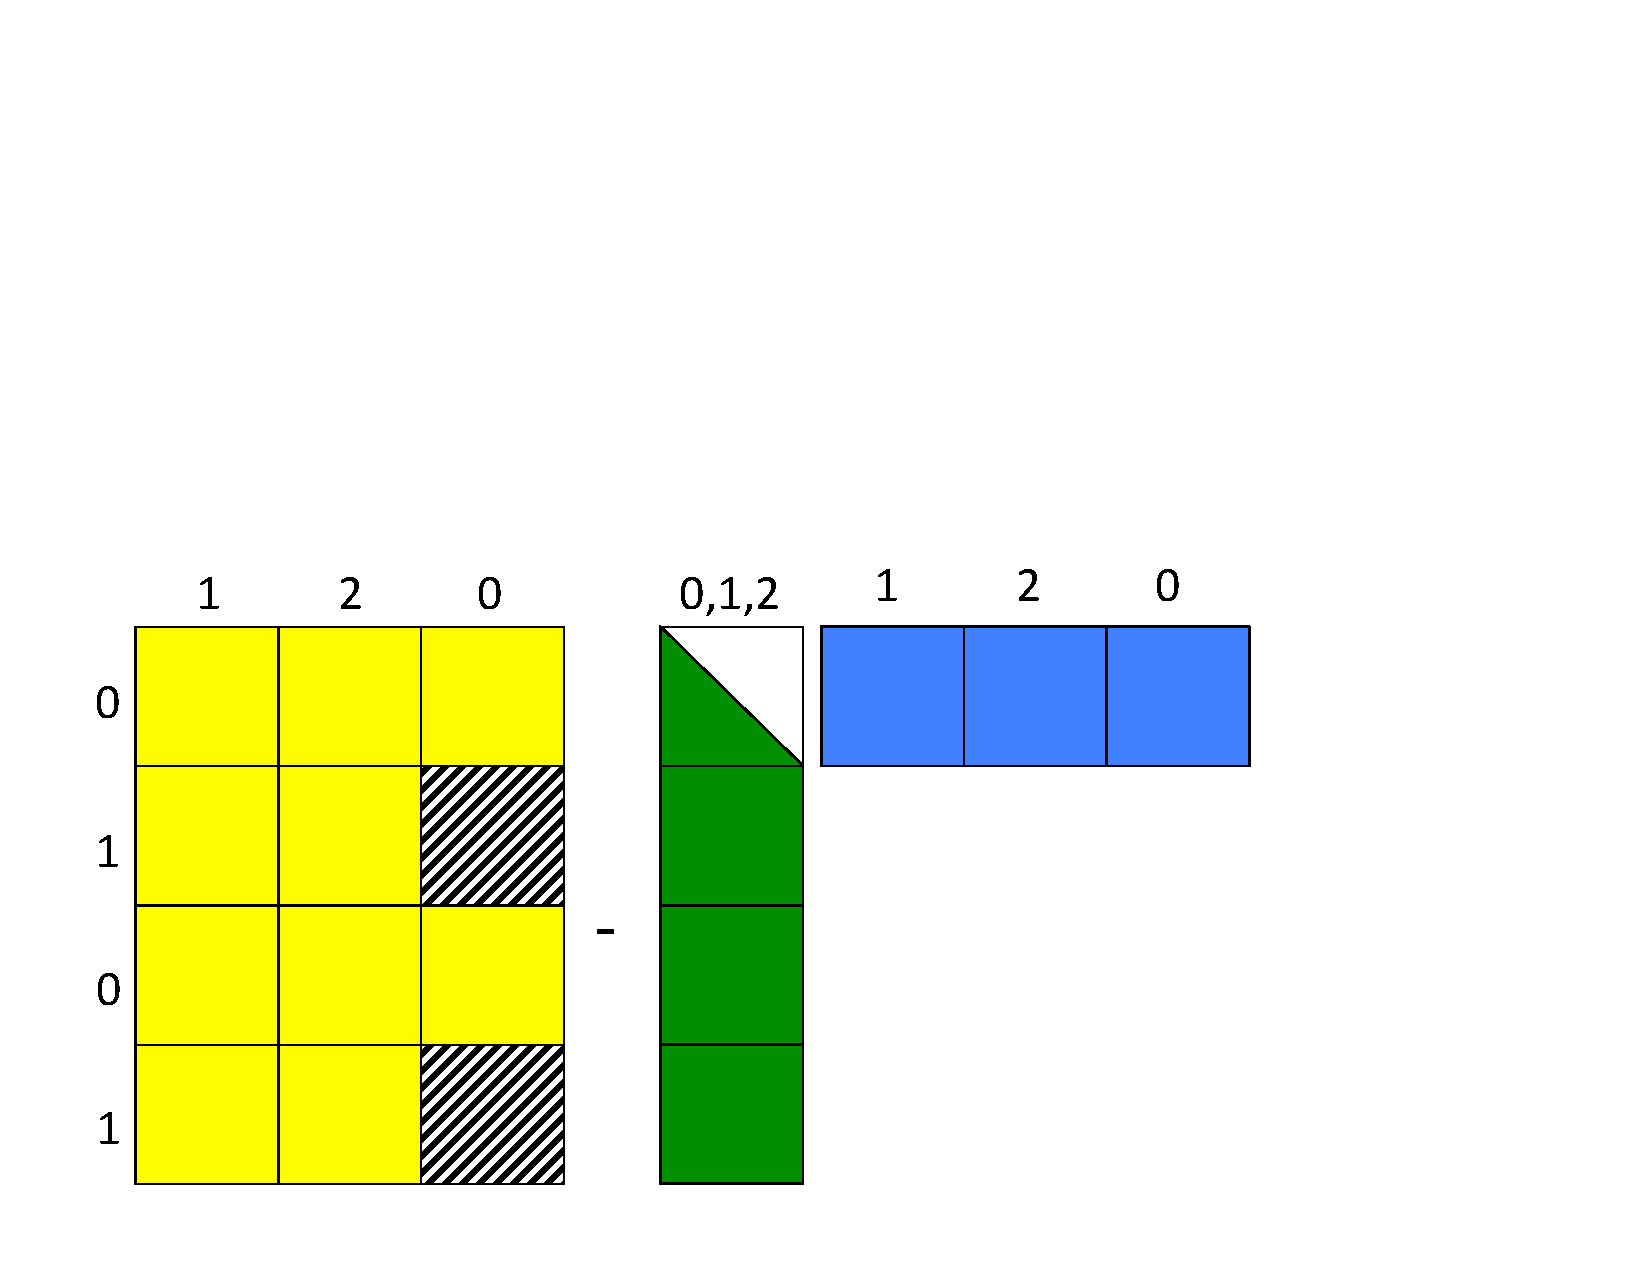
\includegraphics[totalheight=0.15\textheight, width=0.3\textwidth,viewport=10 10 600 360, clip]{figures/pdlarfb_step2}
	\label{fig:pdlarfb_step2}}
	\caption{PDLARFB}
\end{figure}

As shown in Equation (\ref{eqn:qr-trailing}), the trailing update of QR carries
out operation $Q^{T}A_{2}=(I-VT^{T}V^{T})A_{2}\rightarrow
\tilde{A}_{2}$. The right arrow means the updated trailing matrix is
written in-place to $A_{2}$. The trailing matrix update of QR is
similar to PDGEMM for LU which has been shown to hold the checksum
relationship only at the end~\cite{pengduppopp12}. Therefore the procedure
to recover from a failure in PDLARFB is:
\begin{enumerate}
\item Survived processes mark the progress and dump critical data to disk 
\item After re-spawning, all processes dry-run to the failure point
\item All except the replacement process load checkpoint from disk 
\item All processes resume computing from the failure point to the end of PDLARFB
\item At the exit of PDLARFB, recover all lost data in checksum and the whole matrix
\item Execution of PDGEQRF returns to normal
\end{enumerate}
The 'dry-run' step is to re-establish the calling stack of all processes to
the failing point. Therefore PBLAS and ScaLAPACK routines for
computing, for example, PDGEQR2, PDLARFT, etc. are skipped over during 
the dry run.

The recovery is demonstrated with an example of a $4\times 4$ blocks
matrix on a $2\times 3$ grid where failure occurs during PDLARFB.

PDLARFB implements $Q^{T}A_{2}=(I-VT^{T}V^{T})A_{2}$ in three steps:
\begin{enumerate}
\item $W\leftarrow V^{T}A_{2}$
\item $\tilde{W}\leftarrow W\times T$
\item $\tilde{A}_{2}\leftarrow A_{2}-V\tilde{W}^{T}$
\end{enumerate}
Suppose the failure occurs right after step 1 on process (1,0). 
In step 1, as shown in figure~\ref{fig:pdlarfb_step1}, $V$ is stored
in the green trapezoid and $A_{2}$ is in the yellow blocks. $V$ is
first broadcast row-wise to all columns, then GEMM is called on each
process that owns $A_{2}$ with the local $V$ and $A_{2}$. Finally, the
result is produced with column-wise block summation and the result is
stored on the first row of processes that process the first row of
$A_{2}$ (blue blocks).  From the MPI facilities presented in
Section~\ref{sec:mpi}, the failure location is broadcasted to all 
surviving processes and matrix data are dumped to the disk, including
peripheral data like the TAU array and workspace. Surviving processes
also keep a record on whether they have finished the DGEMM in step 1.

After critical data is saved to disk, the program exits and is
re-spawn with a replacement process in the failed process's
location. The re-launched program dry-runs to the failure point in
step 1 of PDLARFB. All previously surviving processes load their
checkpoint from disk while the replacement process stays with its
blank data. Then the program resumes execution of PDLARFB. Since
failure is on process (1,0), $W$ survives the data loss.

Step 2 of PDLARFB is $W\times T$ where $W$ is the blue blocks in
figure~\ref{fig:pdlarfb_step1} and $T$ is a $nb\times nb$ upper
triangular matrix.  Since $T$ resides on each process in the row that
owns $W$, the correctness of $T$ can be always guaranteed, and
therefore $\tilde{W}$ has no lost block in it after calling
DTRMM. $\tilde{W}$ is broadcasted column-wise for step 3.

Step 3 of PDLARFB is shown in figure~\ref{fig:pdlarfb_step2}. In
$\tilde{A}_{2}\leftarrow A_{2}-V\tilde{W}^{T}$, besides
$\tilde{W}^{T}$, $V$ is also correct since $V$ has been broadcast
row-wise to all process in step 1, therefore even if blocks of $V$ are
destroyed by the failure, the result on the replacement process can be
recovered from its neighbor processes in the same row. The result of
step 3, also that of PDLARFB, is affected by the incorrect result in
$A_{2}$, expressed in shadowed blocks in
figure~\ref{fig:pdlarfb_step2}. These incorrect blocks remain in the
result of DGEMM in this step. They are fixed later in the recovery process
in PDGEQRF using both the ABFT and Q-parallel checksum.

For PDLARFB, both $V$ and $T$ can be guaranteed correct no matter when
and where failure occurs, the only variable factor is $W$. However if
the failure does punch holes in $W$, more shadow blocks appear in
the result of PDLARFB, and they can still be fixed by the recovery in
PDGEQRF.
\end{comment}
